\section{Introduction}
Generative modeling is a subset of machine learning that focuses on generating
new data. This is opposed to the more familiar types of models that classify
data, called a discriminative model. This difference in these is that
discriminative models want to find decision boundaries between a set of data
generative models want to learn how to generate data within that boundary. Or
put more mathematically, a discriminative model learns a conditional probability
given a set of data:  $P(Y=\text{label} | X=\text{data})$.
In turn, a generative model tries to produce new data given a set of data:
$P(x)$. In practice a generative model is only approximating the learned
dataset, so we typically write $p_\theta(\hat{x}) \approx p_{true}(x)$. Here we
have $\hat(x)$ represent our training set. We use the hat to indicate that this
set is an subset of the true dataset, as is true for any machine learning
problem. 

With this ability generative models have proven to be able to produce a wide
variety of data, including: images~\cite{}, music~\cite{}, text~\cite{},
voice~\cite{}, and even code~\cite{}. Generative models have also proven useful
for tasks such as: data augmentation~\cite{}, bias identification~\cite{}, data
completion~\cite{}, image upscaling~\cite{}, and compression~\cite{}.

\subsection{Uses of Generative Modeling}
Generative models are most well known for their ability to generate new data.
Websites like \url{ThisPersonDoesNotExist.com} and \url{ThisCatDoesNotExist.com}
have greatly increased the public's familiarity with such machine
learning techniques. Not only can generative models be used to create entirely
but they can also be used to manipulate or augment data. This is commonly
referred to as a deep fake. This type of augmentation can range from changing
a horse to a zebra~\cite{} to replacing the speaker's face~\cite{} and
voice~\cite{} in a video. 

Such form of data augmentation has other uses. A common one is to fill in
missing data. This can range from completing a single set of data as well as
augmenting an entire dataset. The former is useful for tasks like upscaling,
where there is either missing data when an image is upscaled to a higher
resolution~\cite{}, or to fill in missing frames in a video that is upscaled to
a higher framerate. These have had a lot of practical uses for the cinema
industry. Netflix uses this technology to compress their data to reduce their
bandwidth during streaming and also to show movies and shows that were never
filmed in modern resolutions. The gaming industry also uses these techniques to
increase framerates and increase resolution, most notably Nvidia's Deep Learning
Super Sampling (DLSS)~\cite{}. When augmenting an entire dataset, generative
models can be used to reduce bias in the training set~\cite{}. Since it is very
difficult to identify all biases, even in highly tuned datasets, these models
can automatically fill in missing samples. By using this kind of modeling
studies have shown that one can greatly increase the accuracy of the worst
classifying classes within a discriminative model. Thus this reduces key issues
like racial bias in classifiers. 

The other way that generators can uncover bias is by learning the distribution
of data within the training set. Certain kinds of generators learn to
approximate the dataset and by doing this one can look at the tails of the
distribution to understand what areas underperform. This is extremely helpful in
allowing researchers to investigate and better understand the limitations of the
datasets that they use. This is a major issue since the data processing
inequality theorem says that post processing cannot increase information. This
allows researchers to obtain, or generate, new information that can go into the
original dataset and increase the quality of inferences.

\subsection{Types of Generators}
There are many different types of generators that can perform similar tasks in
different ways. We show the taxonomy of generative models, created by Ian
Goodfellow, in Figure~\ref{fig:tax}. 

\begin{figure}[ht]
\centering
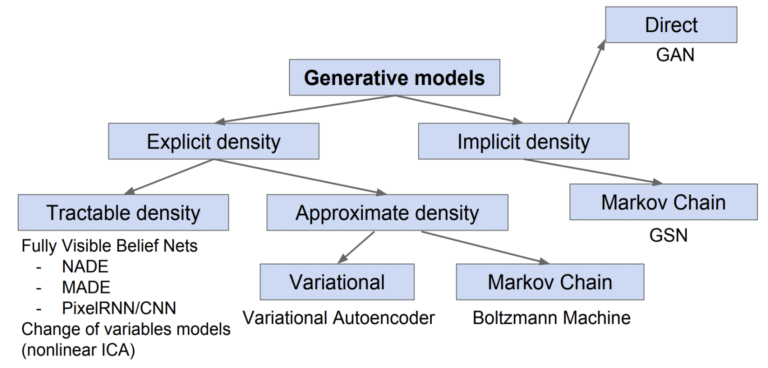
\includegraphics[width=0.48\textwidth]{Taxonomy.png}
\caption{Taxonomy of generative models: Ian Goodfellow}
\label{fig:tax}
\end{figure}

The most important distinction in models is the explicit density estimators vs
the implicit density estimators. In the former case these models explicitly
learn the density function of the dataset. That is, they learn by maximizing the
likelihood function, typically the log-likelihood, as defined by
Equation~\ref{eq:like}. 

\begin{equation}
    L(\theta|x) = \prod f(x_i|\theta)
    \label{eq:like}
\end{equation}

Implicit density estimators do not learn the likelihood
function and just learn a stochastic procedure that directly generates data.
This means that these different methods have different uses. For example, a
implicit method is not going to be well suited for understanding the bias in a
dataset because it is not learning the density function of that dataset. The
implicit method will typically have an advantage in being easier to train and
being more tractable. Unfortunately many problems are not tractable and thus
even explicit methods typically use approximate density estimations. We will
first discuss implicit density estimators and then explicit. In
section~\ref{sec:GAN} we will further discuss Generative Adversarial Networks
and how they work. In sections~\ref{sec:autoencoder} and \ref{sec:vae} we will
discuss autoencoders and variational autoencoders, which are approximate density
estimators. Finally, in section~\ref{sec:nf} we will discuss Normalizing Flows,
which are tractable density estimators.
